% !TeX spellcheck = en_US 
\documentclass[proposal]{byu-aero}

\newcommand{\nextyear}{2021}


%!!!!!!!!!!!!!!!!!!!!!!!!!!!!!!!!!!!!!!!!!!!!!!!!!!!!!!!!!!!!!!!!!!!!!!!!!!!!!!!!!!!!!!!!%
%!!!!!!! UNLESS YOU KNOW WHAT YOU'RE DOING, DO NOT TOUCH ANYTHING ABOVE THIS LINE !!!!!!!%
%!!!!!!!!!!!!!!!!!!!!!!!!!!!!!!!!!!!!!!!!!!!!!!!!!!!!!!!!!!!!!!!!!!!!!!!!!!!!!!!!!!!!!!!!%

%%%%%%%%%%%%%%%%%%%%%%%%%%%%%%%%%%
%%%%%%%%%%   Text Body   %%%%%%%%%
%%%%%%%%%%%%%%%%%%%%%%%%%%%%%%%%%%
\begin{document}

%%%%%%%%%%%%%%%%%%%%%%%%%%%%%%%%%%%%%%%%%%
%%%%%%%%%%   Executive Summary   %%%%%%%%%
%%%%%%%%%%%%%%%%%%%%%%%%%%%%%%%%%%%%%%%%%%
\section{Executive Summary}
\label{sec:ExecutiveSummary}

Our goal is to create a UAV that can transport, deploy, operate, and recover a towed sensor. We are accomplishing this by dividing the design, manufacturing, and reporting of work into various sub-teams, as discussed in section \cref{sec:ManagementSummary}. To ensure that we maximize the points received during flight and ground operations, we performed a design parameter sensitivity analysis which lead us to prioritize a large sensor weight and quick ground operations. The design choices shown in section \cref{sec:ConceptualDesign} reflect these priorities.

Our UAV features a single wing with dual boom and two vertical stabilizers. These design choices enable the stable deployment of the payload without risking damage to the airframe. We have already completed several design iterations of the towed sensor, and have moved on to wind tunnel testing in order to fine tune the aerodynamic stability of our sensor design.

We will also be manufacturing multiple, full-scale prototypes, which will culminate in a stable and sturdy final airframe. Additionally, we will test our propulsion system design using a static thrust stand, validating that our system provides the necessary range and endurance. Furthermore, we will simulate the ground mission to ensure success at the competition.

%%%%%%%%%%%%%%%%%%%%%%%%%%%%%%%%%%%%%%%%%%%
%%%%%%%%%%   Management Summary   %%%%%%%%%
%%%%%%%%%%%%%%%%%%%%%%%%%%%%%%%%%%%%%%%%%%%
\section{Management Summary}
\label{sec:ManagementSummary}
%TEAM ORGANIZATION
\begin{wrapfigure}[7]{R}{0in}
	\centering
	\raisebox{0pt}[\dimexpr\height-3\baselineskip\relax]{
\begin{tikzpicture}[node distance = 1cm, auto]

	% Place nodes
	\node [block] (Project Manager) {\footnotesize Project Manager};
%	\node [block, below left = 0.1 and -1.25cm  of Project Manager] (Engineering Lead) {\footnotesize Engineering Lead};
%	\node [block, below right = 0.1 and -1.25cm   of Project Manager] (Project Manager) {\footnotesize Project Manager};

	\node [block2, below left = 0.25 and -1.25cm of Project Manager] (Aerodynamics) {\footnotesize Aerodynamics};
	\node [block2, below left = 1.0 and -1.25cm  of Project Manager] (Structures) {\footnotesize Structures};
	\node [block2, below left = 1.75 and -1.25cm  of Project Manager] (Propulsion) {\footnotesize Propulsion};
	\node [block2, below right = 0.25 and -1.25cm  of Project Manager] (Systems) {\footnotesize Systems};
	\node [block2, below right = 1.0 and -1.25cm  of Project Manager] (Graphics) {\footnotesize Graphics};
	\node [block2, below right = 1.75 and -1.25cm  of Project Manager] (Manufacturing) {\footnotesize Manufacturing};

	% Draw edges
%	\path[line] let \p1=(Project Manager.south), \p2=(Engineering Lead.east) in (Project Manager.south) --  +(0,0.55*\y2) -| node {} (Engineering Lead.east);
%	\path[line] let \p1=(Project Manager.south), \p2=(Project Manager.west) in (Project Manager.south) -- +(0,0.55*\y2) -| node {} (Project Manager.west);

	\path[line] let \p1=(Project Manager.south), \p2=(Aerodynamics.east) in (Project Manager.south) -- +(0,0.65*\y2) -| node  {} (Aerodynamics.east);
	\path[line] let \p1=(Project Manager.south), \p2=(Systems.west) in (Project Manager.south) -- +(0,0.65*\y2) -| node  {} (Systems.west);

	\path[line] let \p1=(Project Manager.south), \p2=(Structures.east) in (Project Manager.south) -- +(0,0.8*\y2) -| node  {} (Structures.east);
	\path[line] let \p1=(Project Manager.south), \p2=(Graphics.west) in (Project Manager.south) -- +(0,0.8*\y2) -| node  {} (Graphics.west);

	\path[line] let \p1=(Project Manager.south), \p2=(Propulsion.east) in (Project Manager.south) -- +(0,0.85*\y2) -| node  {} (Propulsion.east);
	\path[line] let \p1=(Project Manager.south), \p2=(Manufacturing.west) in (Project Manager.south) -- +(0,0.85*\y2) -| node  {} (Manufacturing.west);
\end{tikzpicture}}
	\caption{Here we show the structure of, and assignment areas within, our team organization.}
	\label{fig:personnelassignments}
\end{wrapfigure}
\begin{table}[h!]
	\centering
	\renewcommand*{\arraystretch}{1.1}
	\caption{Sub-Team Descriptions}
	\label{tab:Roles}
	\rowcolors{2}{BYUbluelite}{white}
	\begin{tabular}{ |m{1.7in}|m{2.5in}|m{2in}| }
		\hline
		\rowcolor{BYUbluemid}
		{Sub-Team} & {Role} & {Required Skills} \\ 
		\hline
		{Aerodynamics} & Calculate performance metrics, stability and important aerodynamic values & MATLAB, XFLR5, familiarity with aerodynamic principles\\
		\hline
		{Structures and CAD} & Create 3D models and design the interior supports and structure & CAD software, introductory structural knowledge\\ 
		\hline
		{Propulsion and Electronics} & Design the electronic systems required to power and sustain the airplane in flight & Knowledge of propulsion and electronic systems including propellers, motors, speed controllers, transmitter, servos, etc. \\ 
		\hline
		{Manufacturing} & Construct and test prototypes. Lead in final construction and assembly of the flight model & Laser cutting, 3D printing, work with different materials and adhesives  \\ 
		\hline
		{Writing} & Lead the writing of the proposal and final report & Technical writing, Microsoft Office, \LaTeX \\
		\hline
	\end{tabular}
\end{table}
This year's BYU Aeronautics Club \textit{Design, Build, Fly} team is designed to focus individual skill sets on relevant tasks. The 10 team members are divided into five sub-teams, with each member expected to work actively on at least two sub-teams. These sub-teams, shown in \cref{fig:Organization Chart}, enable the focusing of skills into accomplishing important work efficiently. Each sub-team is led by a team leader, selected based on their experience in each particular focus area.

The entire team meets weekly to discuss progress on individual sub-teams and the project as a whole. During these meetings assignments are made to the sub-teams, and each sub-team is then responsible to carry out their tasks and to coordinate with other sub-teams as necessary. The weekly meetings ensure that the project is progressing and provides an opportunity for teams to ask for input from other team members. If design conflicts arise between two aspects of the project developed by different sub-teams, then the ultimate decision is made by the sub-team leaders in conjunction with the project lead.


% expanded CO architecture diagram produced by the TikZ package
\documentclass[]{byu-aero}

\def \theyear {2020}
\def \nextyear {2021}

\usepackage[active,tightpage]{preview}
\PreviewEnvironment{tikzpicture}
\setlength{\PreviewBorder}{0em}


%GANTT CHART
\usepackage{pgfgantt}
\ganttset{
	time slot format=isodate,
	time slot unit=day,
	x unit=0.025cm,
	y unit title=0.4cm,
	y unit chart=0.3cm,
	hgrid,
	canvas/.append style={draw=\BYUblue},
	%
	title label font=\bfseries\scriptsize,
	title height=1,
	title/.style={fill=\BYUbluelite,draw=\BYUblue},
	%
	today = \theyear-10-30,
	today label = Current Date,
	today label font=\itshape\tiny,
	today rule/.style={draw=\BYUgray,dashed},
	%
	group/.append style={fill=\BYUbluemid,draw=\BYUblue},
	group top shift=0.25,
	group height=.25,
	group right peak tip position=0.0,
	group left peak tip position=0.0,
	group peaks width=2.0,
	group peaks height=0.25,
	group label font = \bfseries\footnotesize,
	%
	bar/.append style={fill=\BYUblue,draw=\BYUblue},
	bar label font=\footnotesize,
	bar height = 0.25,
	%	bar top shift = 0.25,
	progress label text = {},
	%
	milestone/.append style={fill=\BYUbluelite,draw=\BYUblue,xscale=12},
	milestone height = 0.95,
	milestone top shift = 0.0,
	milestone label font = \itshape\footnotesize,
	%
	%	link/.append style={draw=\BYUblue},
	link tolerance = 10,
	link bulge = 10,
}


\begin{document}
	\begin{figure}[h!]
		\centering
		\begin{ganttchart}[]{\theyear-09-01}{\nextyear-04-30}
			\gantttitlecalendar{year, month=shortname} \\
			%
			%%--DESIGN--%%
			%
			\ganttgroup{Design}{\theyear-09-14}{\nextyear-01-28} \\
			\ganttbar[progress=100]{Conceptual Design}{\theyear-09-14}{\theyear-10-07} \\
			\ganttbar[progress=0]{Preliminary Design}{\theyear-10-31}{\theyear-12-01} \\
			\ganttbar[progress=0]{Detailed Design}{\theyear-12-28}{\nextyear-01-28} \\
			%
			%%--PROTOTYPING--%%
			%
			\ganttgroup{Build}{\theyear-10-01}{\nextyear-02-01} \\
			\ganttbar[progress=100]{Conceptual Prototypes}{\theyear-10-01}{\theyear-10-14} \\
			\ganttbar[progress=0]{Preliminary Prototypes}{\theyear-11-14}{\theyear-12-14} \\
			\ganttbar[progress=0]{Detailed Prototypes}{\nextyear-01-07}{\nextyear-02-01} \\
			\ganttbar[progress=0]{Final Build}{\nextyear-02-20}{\nextyear-03-21}\\
			%
			%%--TESTING--%%
			%
			\ganttgroup{Fly}{\theyear-10-07}{\nextyear-03-28} \\
			\ganttbar[progress=100]{Conceptual Testing}{\theyear-10-07}{\theyear-10-28}\\
			\ganttbar[progress=0]{Preliminary Testing}{\theyear-12-01}{\theyear-12-21}\\
			\ganttbar[progress=0]{Detailed Testing}{\nextyear-01-14}{\nextyear-02-07}\\
			\ganttbar[progress=0]{Practice Runs}{\nextyear-03-21}{\nextyear-03-28}\\
			%
			%%--COMPETING--%%
			%
			\ganttgroup{Competition Milestones}{\theyear-10-30}{\nextyear-04-16} \\
			\ganttmilestone{Submit Proposal}{\theyear-10-30} \\
			\ganttmilestone{Preliminary Design Review}{\theyear-12-21} \\
			\ganttmilestone{Submit Design Report}{\nextyear-02-20} \\
			\ganttmilestone{Submit Proof of Flight}{\nextyear-04-01} \\
			\ganttmilestone{Fly-off}{\nextyear-04-16}
			%
			%
			%%--VERTICAL RULE--%%
%			\ganttvrule[vrule/.append style={draw=\BYUgray}]{\tiny \textit{Current Date}}{\theyear-10-30}
			today=\theyear-10-30
			%
			%%--LINKS--%%
			%
			\ganttlink[link/.append style={draw=\BYUblue}]{elem1}{elem5}
			\ganttlink[link/.append style={draw=\BYUblue}]{elem5}{elem10}
			\ganttlink[link/.append style={draw=\BYUblue}]{elem10}{elem15}
			%
			\ganttlink[link/.append style={draw=\BYUred}]{elem2}{elem6}
			\ganttlink[link/.append style={draw=\BYUred}]{elem6}{elem11}
			\ganttlink[link/.append style={draw=\BYUred}]{elem11}{elem16}
			%
			\ganttlink[link/.append style={draw=\BYUgreen}]{elem3}{elem7}
			\ganttlink[link/.append style={draw=\BYUgreen}]{elem7}{elem12}
			\ganttlink[link/.append style={draw=\BYUgreen}]{elem12}{elem17}
		\end{ganttchart}
	\end{figure}
	
\end{document}

\subsection{Budget}
\label{ssec:budget}

Our prospected project budget is shown in \cref{tab:budget}. Included in our estimates are materials not only for the final aircraft, but also prototyping materials.

% Project Budget
\begin{table}[htb!]
	\centering
	\renewcommand{\arraystretch}{1.2}
	\caption{Project Budget}
	\label{tab:budget}
	\rowcolors{2}{BYUbluelite}{white}
	\begin{tabular}{ |l|l|l| } 
		\hline
		\rowcolor{BYUbluemid}
		Category & Items & Cost (\$) \\ 
		\hline
		Propulsion &  Brushless Motors (x2) | Propellers (x5) | ESCs (x2) & 320 \\
		\hline
		Power & 6S Lipo Batteries (x2) & 100 \\ 
		\hline
		Structures & Balsa Wood | Monokote | ABS Filament (1kg) | Foam & 150 \\ 
		\hline
		Composites & Carbon Fiber Spars (x4) | Fiber Glass | Epoxy & 160  \\ 
		\hline
		Electronics & Servos (x10) | Receiver | Flight Controller & 110 \\
		\hline
		Travel & Vehicle Rental | Gas (6 Members) & 450 \\
		\hline
		Lodging & Airbnb (6 Members) & 900 \\
		\hline 
		\textbf{Total} & & \textbf{2190} \\ 
		\hline
		
	\end{tabular}
\end{table}

%%%%%%%%%%%%%%%%%%%%%%%%%%%%%%%%%%%%%%%%%%
%%%%%%%%%%   Conceptual Design   %%%%%%%%%
%%%%%%%%%%%%%%%%%%%%%%%%%%%%%%%%%%%%%%%%%%
\section{Conceptual Design Approach}
\label{sec:ConceptualDesign}


\subsection{Mission Requirements}
\label{ssec:missionreqs}
The aircraft must complete a ground mission and three flight missions as follows: 

\noindent \textbf{Ground Mission:} The assembly crew team member must demonstrate payload accessibility, sensor resilience, and the sensor deployment/recovery mechanism functionality. The score is based on the time required to complete the ground mission. 

\noindent \textbf{Flight Mission 1:} Staging flight: the aircraft must complete 3 laps of the competition course within a 5-minute window. One point is awarded for a successful flight. 

\noindent \textbf{Flight Mission 2:} Delivery Flight: The aircraft will carry its maximum payload (sensor in shipping container, shipping container simulators, and deployment/recovery mechanism). The score is a function of the number of shipping containers carried, divided by the time required to fly 3 laps. An additional point is awarded for completing the mission. 

\noindent \textbf{Flight Mission 3:} Sensor Flight: The aircraft will carry the sensor and the deployment/recovery mechanism. The aircraft will deploy the sensor, complete as many laps as possible in a 10-minute window, then recover the sensor and complete a successful landing. The mission score is the product of the number of laps flown, the sensor length, and the sensor weight. An additional two points are awarded for completing the mission.

\subsection{Sensitivity Studies}
\label{ssec:sensitivitystudies}

\begin{wrapfigure}[9]{R}{7.5cm}
	\centering
	\vspace*{-10pt}
	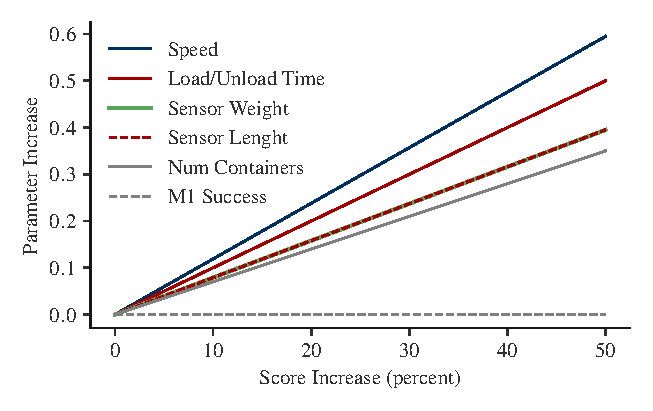
\includegraphics[width = 0.4\textwidth]{sensitivity}
	\caption{The sensitivity study of parameters.}
	\label{fig:Sensitivity Analysis}
\end{wrapfigure}
We analyzed the sensitivity of the total mission score to design parameters. To simplify the analysis, we considered the scoring factors of Time from Mission 2 and Number of Laps from Mission 3 into a single design outcome: Speed. We discussed the collateral effects of the remaining scoring factors on the others, and decided to conduct our sensitivity analysis as if they were independent factors.

According to the results of our sensitivity analysis, shown in \cref{fig:Sensitivity Analysis}, the most important factors are the airplane speed and the time required to complete the Ground Mission. Therefore, our design will prioritize speed and easy access to the airplane cargo bay. Additionally, we decided to increase the sensor weight and decrease the number of packages to increase our score on the second mission. This also results in a faster load/unload time for the Ground Mission.

\subsection{Preliminary Design}
\label{ssec:preliminarydesign}

\begin{figure}[h!]
	\centering
	\begin{subfigure}[t]{0.45\textwidth} % width of left subfigure
		\centering
	    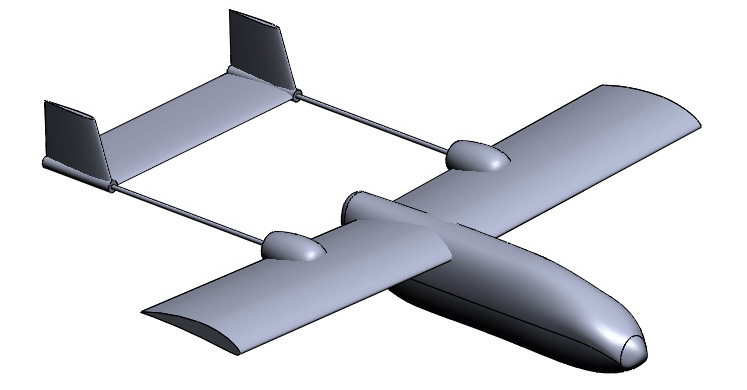
\includegraphics[width=\textwidth]{CADModel}
		\caption{A CAD model of our current design iteration.}
		\label{fig:CAD Model}
	\end{subfigure}
	\hfill
	\begin{subfigure}[t]{0.45\textwidth} % width of right subfigure
		\centering
		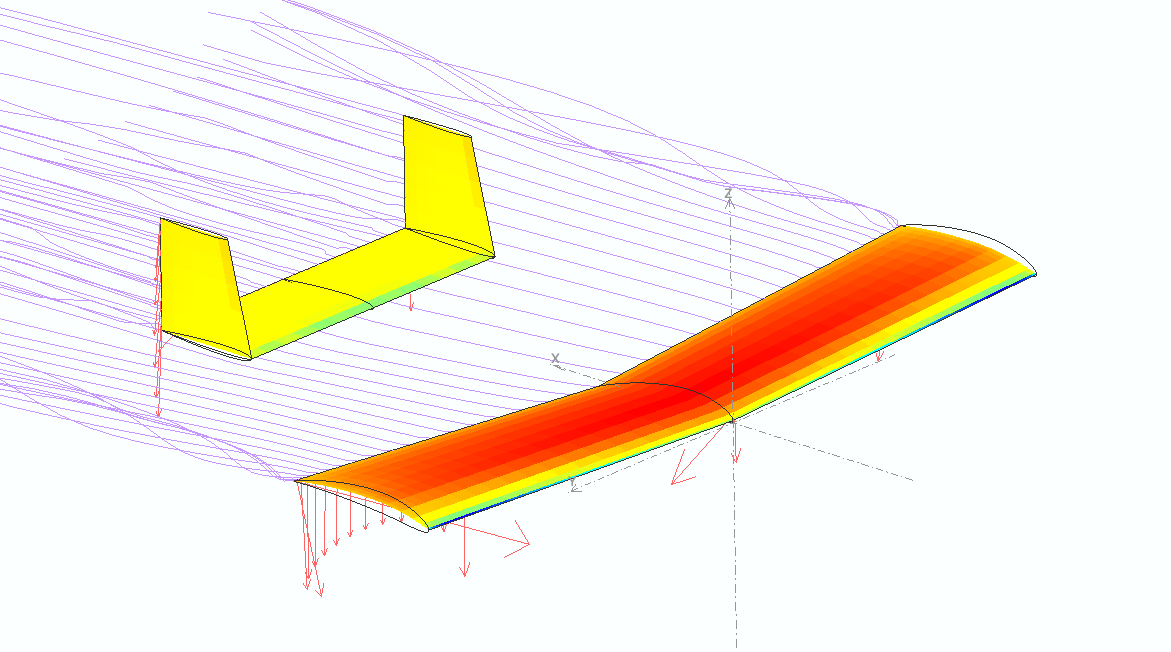
\includegraphics[width=\textwidth]{XFLR5Model.png}
		\caption{An XFLR5 analysis of our design showing the pressure distribution, wake, and downwash.}
		\label{fig:XFLR5 Model}
	\end{subfigure}
	\caption{Images of our preliminary design.}
	\label{fig:prelimdesign}
\end{figure}


Our design objectives are to maximize vehicle air speed and minimize the cargo load/unload time. The following preliminary design is crafted to meet those objectives. As we continue testing, we will make further improvements to the design.

\noindent \textbf{Configuration:} We decided to use a single wing with a twin-boom tail. After researching the a biplane configuration to maximize lift, we decided that a monoplane would be simpler and more stable, as well as enabling easier modular construction. The twin boom tail design allows the sensor to be deployed out the back of the fuselage without risk of damaging the tail and airframe.


\noindent \textbf{Wing Geometry:} Our wing was designed to achieve our goal of maximizing sensor weight, with the current iteration being designed to carry 10 lbs. We performed aerodynamic analyses using XFLR5, leading the aerodynamics sub-team to select a 12-inch chord and the NACA 6412 airfoil for the entire wing. To further improve the lift, we mount wing at an angle of attack of \(3^\circ\). We improved stability by using a \(3^\circ\) dihedral and a \(5^\circ\) root-tip washout. This configuration has a cruise speed of 48 mph with a 10 lb. takeoff weight.

\noindent \textbf{Tail Design:} The aerodynamics team determined that a “U” tail will maximize stability, ground clearance, and structural rigidity, especially with the twin boom design. The tail uses NACA 0009 airfoils for both the horizontal and vertical stabilizers.


\begin{figure}[h!]
	\centering
	\begin{subfigure}[t]{0.475\textwidth} % width of left subfigure
		\centering
		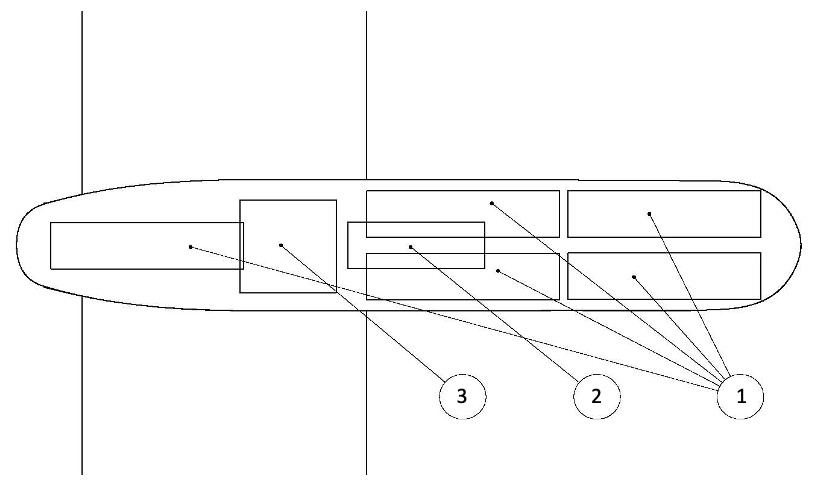
\includegraphics[width=3in]{InteriorTopView.png}
		\caption{Top-down view of fuselage.}
		\label{fig:chorddist}
	\end{subfigure}
	\hfill
	\begin{subfigure}[t]{0.475\textwidth} % width of right subfigure
		\centering
		 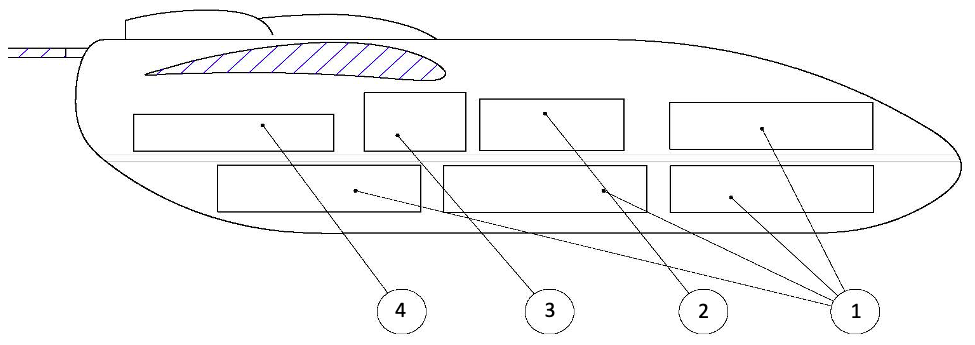
\includegraphics[width=3in]{InteriorSideView.png}
		\caption{Side view of fuselage.}
		\label{fig:twistdist}
	\end{subfigure}
	\caption{Interior views of the fuselage. Numbers correspond to 1) Shipping Containers, 2) Battery, 3) Winch Mechanism, and 4) Electronics.}
	\label{fig:rotorgeom}
\end{figure}

\begin{wrapfigure}[6]{R}{6.5cm}
	\centering
	\vspace*{-14pt}
	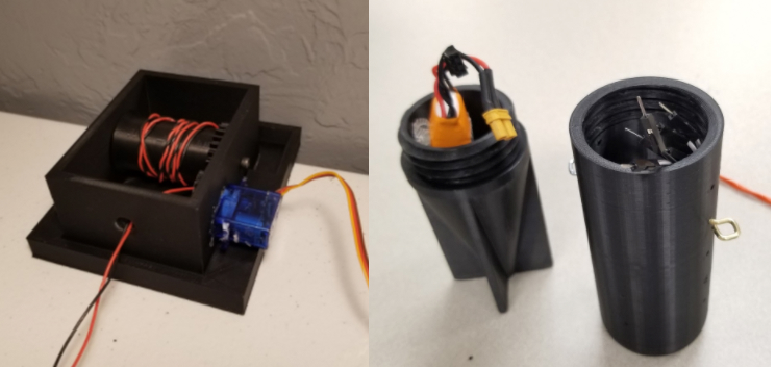
\includegraphics[width=2.0in]{payload}
	\caption{Current sensor rig: winch on left, towed sensor assembly on right}
	\label{fig:Payload CAD}
\end{wrapfigure}

\vspace*{-1em}

\noindent \textbf{Fuselage:} The payload and propulsion teams determined that a streamlined box-style fuselage would be most effective for our priorities. We designed the fuselage with sufficient internal space for all necessary electronic components, mechanisms, and payload. Our fuselage design also facilitates balance adjustments to more easily achieve static stability.

\noindent \textbf{Payload:} We have already completed several design iterations for the towed sensor. We have used wind tunnel tests to explore various tow lines and tow locations along the sensor. In upcoming design iterations we will explore increasing the drag at the back of the sensor, similar to towed radar decoys used by military jets. An image of our current design is shown in \cref{fig:Payload CAD}.

The deployment/recovery mechanism includes a 3D-printed winch connected to a metal geared servo motor. The winch is designed with a quick release base to facilitate quick installation and removal in order to decrease ground mission time. The control wires of the sensor pod will also serve as a tow line. 
%The functions of the sensor are controlled by an Arduino Nano which includes a printed circuit board containing LED circuitry, overcurrent protection, and noise cancellation.

%%%%%%%%%%%%%%%%%%%%%%%%%%%%%%%%%%%%%%%%%%%
%%%%%%%%%%   Manufacturing Plan   %%%%%%%%%
%%%%%%%%%%%%%%%%%%%%%%%%%%%%%%%%%%%%%%%%%%%
\section{Manufacturing Plan}
\label{sec:manufacturing}

The manufacturing team will construct CNC hotwire-cut foam-core wings, pine dowel tail booms, and a foam board fuselage. They will reinforce high stress areas with basswood and composite materials. We will use initial prototypes to acquire useful empirical data about the structure and flight performance of our design.

We plan to construct the wings and tail of the final model from balsa wood, the fuselage from balsa and composite materials, and the tail booms from carbon fiber dowels. We will fabricate various structural and functional parts from laser cut wood, and 3D printed plastics as well.

\begin{figure}[h!]
	\centering
	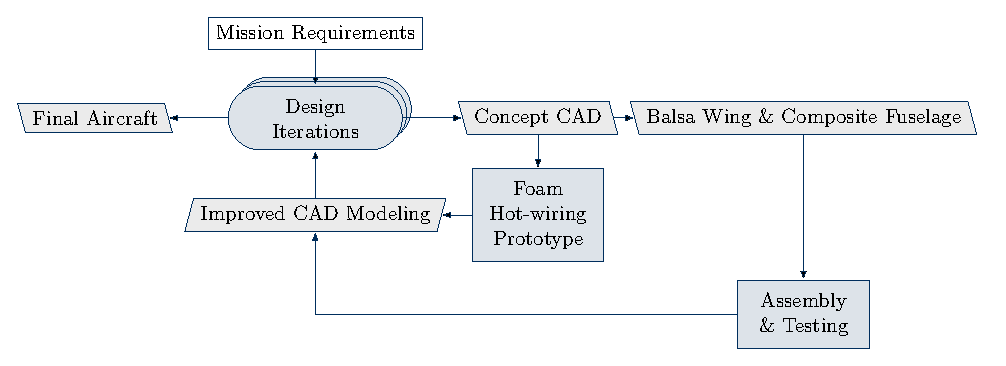
\includegraphics[width=4.5in]{manufacturing_flow.pdf}
	\caption{We show here a flowchart of our proposed manufacturing plan.}
	\label{fig:manufacturingplan}
\end{figure}

%%%%%%%%%%%%%%%%%%%%%%%%%%%%%%%%%%%%%
%%%%%%%%%%   Testing Plan   %%%%%%%%%
%%%%%%%%%%%%%%%%%%%%%%%%%%%%%%%%%%%%%
\vspace*{-1em}
 \section{Testing Plan}
 \label{sec:TestingPlan}

\subsection{Component and Ground Test Plan}

Each team will regularly perform tests on their sub-systems during the design and revision process. The payload team will wind tunnel test the sensor pod to evaluate and improve aerodynamic stability at airspeeds within the flight envelope.  The structures team will perform taxi and drop tests on the landing gear to ensure functionality. They will also conduct physical load tests on the main wing to ensure that the airframe can withstand flight forces. Using a static thrust stand, the propulsion team will evaluate the current draw and static thrust of several combinations of motors, batteries, and propellers to maximize flight speed and duration within our objective flight envelope. We will additionally perform simulations of the ground mission to evaluate the accessibility of the fuselage as well as practice and improve our performance for the competition.

\subsection{Flight Test Plan}

Foam prototype construction allows for high speed prototyping to test and refine the airframe using real world flight tests over several design iterations. Early prototypes of the full aircraft will be tested from late November through January (see \cref{fig:plannedtiming}).  After we have validated our full design (to be completed by January), we will perform flight tests with a balsa wood and composite final model. We will gather data via the pilot's perspective and from on-board sensors for all flight tests to evaluate and improve flight performance.

%%%%%%%%%%%%%%%%%%%%%%%%%%%%%%%%%%%%%
%%%%%%%%%%   Bibliography   %%%%%%%%%
%%%%%%%%%%%%%%%%%%%%%%%%%%%%%%%%%%%%%
%Bibliography (5 Points)
%\item List of all published works referenced in the text must be present in this section.
%\item Any material taken from a published source in all previous sections must have a numerical subscript corresponding to the appropriate citation in this section.
%\item References should appear in numerical order.
%\item Format should match AIAA provided guidelines:
%\newpage
%\clearpage
%\bibliography{ref}{}
%\bibliographystyle{aiaa}

\end{document}
